\subsubsection{Action Obfuscator} \label{subsubsectionection:counter-replace-encryption-content-obfuscator}
The second approach
\begin{figure}[h]
    \centering
    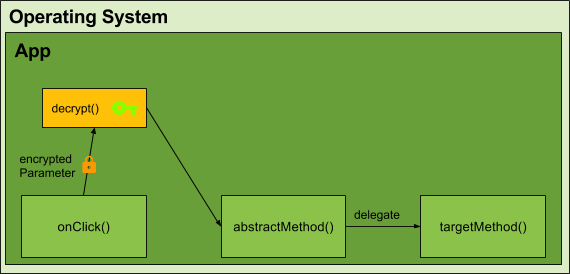
\includegraphics[width=0.8\textwidth]{data/encryptionAction.png}
    \caption{Encrypted actions to obfuscate dependencies}
    \label{fig:encryptionAction}
\end{figure}

e.g. initiate action 1 but add 1 and encrypt (obfscation)

nicht für boolean

default or random action in case decryption is not working or disabled
